\documentclass{spiral-kurs}
\def\title{Sad}
\def\id{sad}
\def\TL{2~s}
\def\ML{256~MB}
\begin{document}
\makeheader
%
  Pan Jan jest właścicielem sadu, w którym rosną piękne jabłonie.
  Aby zabezpieczyć swoje zbiory jabłek, chciałby on ogrodzić sad prostokątnym płotem.

  Dla uproszczenia każdą z jabłoni utożsamiamy z pewnym punktem na płaszczyźnie.
  Płot ma mieć kształt prostokąta o bokach równoległych do osi układu współrzędnych.
  Koszt postawienia płotu zależy od jego długości.
  Pomóż Panu Janowi wyznaczyć prostokątny płot o minimalnym obwodzie, zawierający wszystkie jabłonie.
  Napisz program, który wypisze ten obwód.

  \section{Wejście}
W pierwszym wierszu wejścia znajduje się jedna liczba naturalna $n$ ($2\le n\le 100\,000$),
oznaczająca liczbę jabłoni.
Każdy z kolejnych $n$ wierszy zawiera dwie liczby całkowite $x_i$, $y_i$
($0\le x_i,y_i\le 1\,000\,000$), oddzielone pojedynczym odstępem i oznaczające
współrzędne $i$-tej jabłoni.
Żadne dwie jabłonie nie znajdują się w tym samym punkcie.

\section{Wyjście}
Pierwszy i jedyny wiersz wyjścia powinien zawierać jedną liczbę naturalną oznaczającą
minimalny obwód prostokąta o bokach równoległych do osi układu współrzędnych,
w którym mieszczą się wszystkie punkty podane na wejściu.
Każdy punkt musi leżeć we wnętrzu bądź na brzegu prostokąta.
Możesz założyć, że wynikowy prostokąt będzie miał dodatnie pole.


    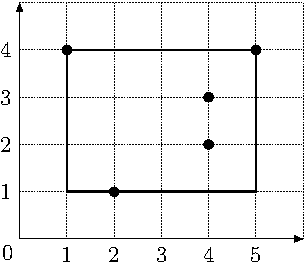
\includegraphics{sadrys-crop}
    \example{0}


  \end{document}
